\documentclass[twoside]{book}

% Packages required by doxygen
\usepackage{calc}
\usepackage{doxygen}
\usepackage{graphicx}
\usepackage[utf8]{inputenc}
\usepackage{makeidx}
\usepackage{multicol}
\usepackage{multirow}
\usepackage{textcomp}
\usepackage[table]{xcolor}

% Font selection
\usepackage[T1]{fontenc}
\usepackage{mathptmx}
\usepackage[scaled=.90]{helvet}
\usepackage{courier}
\usepackage{amssymb}
\usepackage{sectsty}
\renewcommand{\familydefault}{\sfdefault}
\allsectionsfont{%
  \fontseries{bc}\selectfont%
  \color{darkgray}%
}
\renewcommand{\DoxyLabelFont}{%
  \fontseries{bc}\selectfont%
  \color{darkgray}%
}

% Page & text layout
\usepackage{geometry}
\geometry{%
  a4paper,%
  top=2.5cm,%
  bottom=2.5cm,%
  left=2.5cm,%
  right=2.5cm%
}
\tolerance=750
\hfuzz=15pt
\hbadness=750
\setlength{\emergencystretch}{15pt}
\setlength{\parindent}{0cm}
\setlength{\parskip}{0.2cm}
\makeatletter
\renewcommand{\paragraph}{%
  \@startsection{paragraph}{4}{0ex}{-1.0ex}{1.0ex}{%
    \normalfont\normalsize\bfseries\SS@parafont%
  }%
}
\renewcommand{\subparagraph}{%
  \@startsection{subparagraph}{5}{0ex}{-1.0ex}{1.0ex}{%
    \normalfont\normalsize\bfseries\SS@subparafont%
  }%
}
\makeatother

% Headers & footers
\usepackage{fancyhdr}
\pagestyle{fancyplain}
\fancyhead[LE]{\fancyplain{}{\bfseries\thepage}}
\fancyhead[CE]{\fancyplain{}{}}
\fancyhead[RE]{\fancyplain{}{\bfseries\leftmark}}
\fancyhead[LO]{\fancyplain{}{\bfseries\rightmark}}
\fancyhead[CO]{\fancyplain{}{}}
\fancyhead[RO]{\fancyplain{}{\bfseries\thepage}}
\fancyfoot[LE]{\fancyplain{}{}}
\fancyfoot[CE]{\fancyplain{}{}}
\fancyfoot[RE]{\fancyplain{}{\bfseries\scriptsize Generated on Tue Sep 10 2013 13:39:43 for HMC_BNN by Doxygen }}
\fancyfoot[LO]{\fancyplain{}{\bfseries\scriptsize Generated on Tue Sep 10 2013 13:39:43 for HMC_BNN by Doxygen }}
\fancyfoot[CO]{\fancyplain{}{}}
\fancyfoot[RO]{\fancyplain{}{}}
\renewcommand{\footrulewidth}{0.4pt}
\renewcommand{\chaptermark}[1]{%
  \markboth{#1}{}%
}
\renewcommand{\sectionmark}[1]{%
  \markright{\thesection\ #1}%
}

% Indices & bibliography
\usepackage{natbib}
\usepackage[titles]{tocloft}
\setcounter{tocdepth}{3}
\setcounter{secnumdepth}{5}
\makeindex

% Hyperlinks (required, but should be loaded last)
\usepackage{ifpdf}
\ifpdf
  \usepackage[pdftex,pagebackref=true]{hyperref}
\else
  \usepackage[ps2pdf,pagebackref=true]{hyperref}
\fi
\hypersetup{%
  colorlinks=true,%
  linkcolor=blue,%
  citecolor=blue,%
  unicode%
}

% Custom commands
\newcommand{\clearemptydoublepage}{%
  \newpage{\pagestyle{empty}\cleardoublepage}%
}


%===== C O N T E N T S =====

\begin{document}

% Titlepage & ToC
\hypersetup{pageanchor=false}
\pagenumbering{roman}
\begin{titlepage}
\vspace*{7cm}
\begin{center}%
{\Large H\-M\-C\-\_\-\-B\-N\-N \\[1ex]\large 1 }\\
\vspace*{1cm}
{\large Generated by Doxygen 1.8.4}\\
\vspace*{0.5cm}
{\small Tue Sep 10 2013 13:39:43}\\
\end{center}
\end{titlepage}
\clearemptydoublepage
\tableofcontents
\clearemptydoublepage
\pagenumbering{arabic}
\hypersetup{pageanchor=true}

%--- Begin generated contents ---
\chapter{Hierarchical Index}
\section{Class Hierarchy}
This inheritance list is sorted roughly, but not completely, alphabetically\-:\begin{DoxyCompactList}
\item \contentsline{section}{H\-M\-C\-\_\-base}{\pageref{class_h_m_c__base}}{}
\begin{DoxyCompactList}
\item \contentsline{section}{B\-N\-N\-\_\-regression}{\pageref{class_b_n_n__regression}}{}
\item \contentsline{section}{H\-M\-C\-\_\-dist}{\pageref{class_h_m_c__dist}}{}
\end{DoxyCompactList}
\end{DoxyCompactList}

\chapter{Data Structure Index}
\section{Data Structures}
Here are the data structures with brief descriptions\-:\begin{DoxyCompactList}
\item\contentsline{section}{\hyperlink{class_b_n_n__regression}{B\-N\-N\-\_\-regression} \\*B\-N\-N functional approximation class }{\pageref{class_b_n_n__regression}}{}
\item\contentsline{section}{\hyperlink{class_h_m_c__base}{H\-M\-C\-\_\-base} \\*Base Hybrid Monte Carlo class }{\pageref{class_h_m_c__base}}{}
\item\contentsline{section}{\hyperlink{class_h_m_c__dist}{H\-M\-C\-\_\-dist} \\*Probability distribution class }{\pageref{class_h_m_c__dist}}{}
\end{DoxyCompactList}

\chapter{File Index}
\section{File List}
Here is a list of all files with brief descriptions\-:\begin{DoxyCompactList}
\item\contentsline{section}{include/\hyperlink{_b_n_n__regression_8h}{B\-N\-N\-\_\-regression.\-h} }{\pageref{_b_n_n__regression_8h}}{}
\item\contentsline{section}{include/\hyperlink{define__type_8h}{define\-\_\-type.\-h} }{\pageref{define__type_8h}}{}
\item\contentsline{section}{include/\hyperlink{_h_m_c__base_8h}{H\-M\-C\-\_\-base.\-h} }{\pageref{_h_m_c__base_8h}}{}
\item\contentsline{section}{include/\hyperlink{_h_m_c__dist_8h}{H\-M\-C\-\_\-dist.\-h} }{\pageref{_h_m_c__dist_8h}}{}
\item\contentsline{section}{src/\hyperlink{_b_n_n__regression_8cc}{B\-N\-N\-\_\-regression.\-cc} }{\pageref{_b_n_n__regression_8cc}}{}
\item\contentsline{section}{src/\hyperlink{_h_m_c_8cxx}{H\-M\-C.\-cxx} }{\pageref{_h_m_c_8cxx}}{}
\item\contentsline{section}{src/\hyperlink{_h_m_c__base_8cc}{H\-M\-C\-\_\-base.\-cc} }{\pageref{_h_m_c__base_8cc}}{}
\item\contentsline{section}{src/\hyperlink{multidimprob_8cc}{multidimprob.\-cc} }{\pageref{multidimprob_8cc}}{}
\end{DoxyCompactList}

\chapter{Data Structure Documentation}
\hypertarget{class_b_n_n__regression}{\section{B\-N\-N\-\_\-regression Class Reference}
\label{class_b_n_n__regression}\index{B\-N\-N\-\_\-regression@{B\-N\-N\-\_\-regression}}
}


B\-N\-N functional approximation class.  




{\ttfamily \#include \char`\"{}B\-N\-N\-\_\-regression.\-h\char`\"{}}

Inheritance diagram for B\-N\-N\-\_\-regression\-:\begin{figure}[H]
\begin{center}
\leavevmode
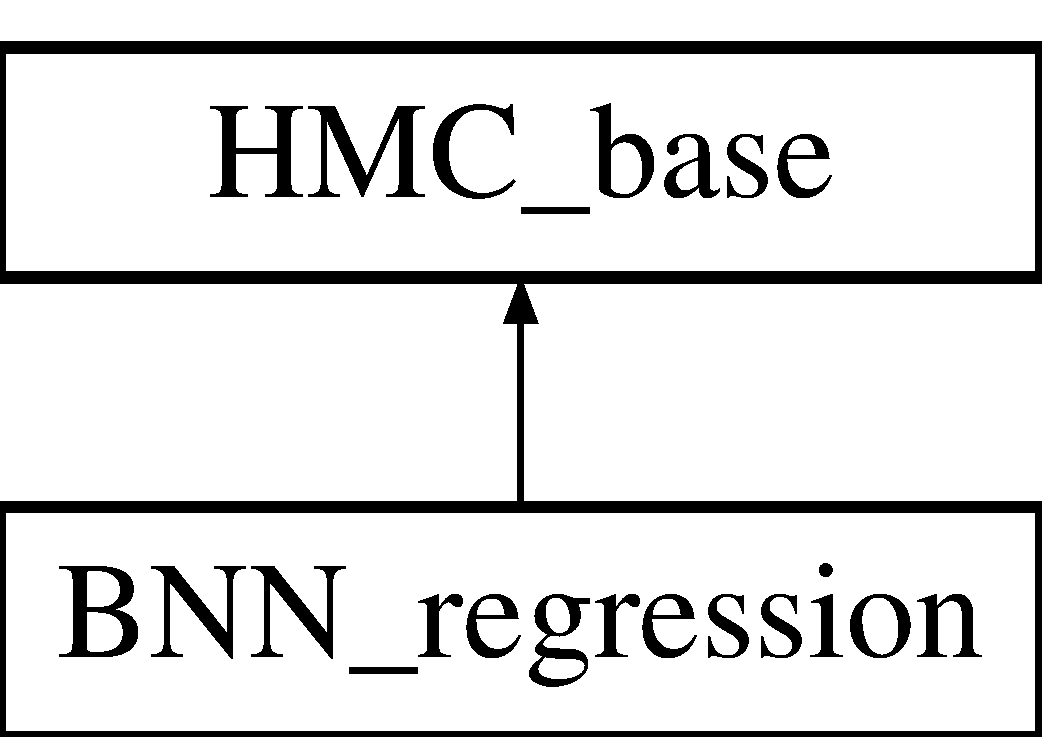
\includegraphics[height=2.000000cm]{class_b_n_n__regression}
\end{center}
\end{figure}
\subsection*{Public Member Functions}
\begin{DoxyCompactItemize}
\item 
\hyperlink{class_b_n_n__regression_acc1e541db00ddc40d6d1038b3e757f99}{B\-N\-N\-\_\-regression} (int l, int h, int i)
\item 
\hyperlink{class_b_n_n__regression_a0096fd7a59f8b57dea848bf3a8df8c7d}{B\-N\-N\-\_\-regression} (int l, int h, int i, std\-::vector$<$ \hyperlink{define__type_8h_a9adf655d34223b34db3baff5c7ce420c}{H\-M\-C\-\_\-type} $>$ \&data, std\-::vector$<$ \hyperlink{define__type_8h_a9adf655d34223b34db3baff5c7ce420c}{H\-M\-C\-\_\-type} $>$ \&targets, std\-::vector$<$ \hyperlink{define__type_8h_a9adf655d34223b34db3baff5c7ce420c}{H\-M\-C\-\_\-type} $>$ \&weights)
\item 
virtual \hyperlink{class_b_n_n__regression_a6a47225939e7f7b9c33d415f315abc48}{$\sim$\-B\-N\-N\-\_\-regression} ()
\item 
virtual \hyperlink{define__type_8h_a9adf655d34223b34db3baff5c7ce420c}{H\-M\-C\-\_\-type} \hyperlink{class_b_n_n__regression_a57303ef1ca25e08c7489fb5095f23527}{U} (std\-::vector$<$ \hyperlink{define__type_8h_a9adf655d34223b34db3baff5c7ce420c}{H\-M\-C\-\_\-type} $>$ \&)
\item 
virtual std\-::vector$<$ \hyperlink{define__type_8h_a9adf655d34223b34db3baff5c7ce420c}{H\-M\-C\-\_\-type} $>$ \hyperlink{class_b_n_n__regression_a779b2feff8192046b2670e80b88547ba}{del\-U} (std\-::vector$<$ \hyperlink{define__type_8h_a9adf655d34223b34db3baff5c7ce420c}{H\-M\-C\-\_\-type} $>$ \&)
\item 
void \hyperlink{class_b_n_n__regression_aec01e7a9c47f666909699e8e50dad2e4}{add} (std\-::vector$<$ \hyperlink{define__type_8h_a9adf655d34223b34db3baff5c7ce420c}{H\-M\-C\-\_\-type} $>$ \&input, \hyperlink{define__type_8h_a9adf655d34223b34db3baff5c7ce420c}{H\-M\-C\-\_\-type} target, \hyperlink{define__type_8h_a9adf655d34223b34db3baff5c7ce420c}{H\-M\-C\-\_\-type} weight=1)
\end{DoxyCompactItemize}
\subsection*{Private Member Functions}
\begin{DoxyCompactItemize}
\item 
\hyperlink{define__type_8h_a9adf655d34223b34db3baff5c7ce420c}{H\-M\-C\-\_\-type} \hyperlink{class_b_n_n__regression_a0f6edf9b223a6aa5fff75b9678592500}{f} (std\-::vector$<$ \hyperlink{define__type_8h_a9adf655d34223b34db3baff5c7ce420c}{H\-M\-C\-\_\-type} $>$ \&, int)
\begin{DoxyCompactList}\small\item\em neural network function \end{DoxyCompactList}\item 
\hyperlink{define__type_8h_a9adf655d34223b34db3baff5c7ce420c}{H\-M\-C\-\_\-type} \hyperlink{class_b_n_n__regression_ac1006eb66df1e5a874c47eb1dae22c81}{Ln\-Prior} (std\-::vector$<$ \hyperlink{define__type_8h_a9adf655d34223b34db3baff5c7ce420c}{H\-M\-C\-\_\-type} $>$ \&)
\begin{DoxyCompactList}\small\item\em Log\-Prior function. \end{DoxyCompactList}\end{DoxyCompactItemize}
\subsection*{Private Attributes}
\begin{DoxyCompactItemize}
\item 
std\-::vector$<$ \hyperlink{define__type_8h_a9adf655d34223b34db3baff5c7ce420c}{H\-M\-C\-\_\-type} $>$ \hyperlink{class_b_n_n__regression_a81f1e9e60fc0c057a99687ec6be99c6e}{x}
\begin{DoxyCompactList}\small\item\em training data \end{DoxyCompactList}\item 
int \hyperlink{class_b_n_n__regression_a0f200c3e1f769b7f7287751dbb9a879d}{H}
\begin{DoxyCompactList}\small\item\em number of hidden nodes \end{DoxyCompactList}\item 
int \hyperlink{class_b_n_n__regression_a134c65919bfa6fb8cb784c9398be3230}{I}
\begin{DoxyCompactList}\small\item\em number of data inputs \end{DoxyCompactList}\item 
int \hyperlink{class_b_n_n__regression_af6ab772dcedde86e69cfd29cb3115387}{N}
\begin{DoxyCompactList}\small\item\em number of training events \end{DoxyCompactList}\item 
\hyperlink{define__type_8h_a9adf655d34223b34db3baff5c7ce420c}{H\-M\-C\-\_\-type} \hyperlink{class_b_n_n__regression_a9f95130775752bea784e043d832945c1}{sig}
\begin{DoxyCompactList}\small\item\em standard deviation for priors \end{DoxyCompactList}\item 
std\-::vector$<$ \hyperlink{define__type_8h_a9adf655d34223b34db3baff5c7ce420c}{H\-M\-C\-\_\-type} $>$ \hyperlink{class_b_n_n__regression_a950982785131b5e7945742ef40dd5860}{w}
\begin{DoxyCompactList}\small\item\em training event weights \end{DoxyCompactList}\item 
std\-::vector$<$ \hyperlink{define__type_8h_a9adf655d34223b34db3baff5c7ce420c}{H\-M\-C\-\_\-type} $>$ \hyperlink{class_b_n_n__regression_aa99d3e95fd4751552cbafec043b4b27d}{t}
\begin{DoxyCompactList}\small\item\em targets for training data \end{DoxyCompactList}\item 
\hyperlink{define__type_8h_a9adf655d34223b34db3baff5c7ce420c}{H\-M\-C\-\_\-type} \hyperlink{class_b_n_n__regression_a6c793005c574b73cfe7d0e1776c21c52}{sigb}
\begin{DoxyCompactList}\small\item\em standard deviation for b parameters \end{DoxyCompactList}\item 
\hyperlink{define__type_8h_a9adf655d34223b34db3baff5c7ce420c}{H\-M\-C\-\_\-type} \hyperlink{class_b_n_n__regression_af06eef668a70e92a122b185c55003b66}{sigv}
\begin{DoxyCompactList}\small\item\em standard deviation for v parameters \end{DoxyCompactList}\item 
\hyperlink{define__type_8h_a9adf655d34223b34db3baff5c7ce420c}{H\-M\-C\-\_\-type} \hyperlink{class_b_n_n__regression_a608b84f81e365e0fd18662583982bc1f}{siga}
\begin{DoxyCompactList}\small\item\em standard deviation for a parameters \end{DoxyCompactList}\item 
\hyperlink{define__type_8h_a9adf655d34223b34db3baff5c7ce420c}{H\-M\-C\-\_\-type} \hyperlink{class_b_n_n__regression_ac7097e88870f47f312e8de1c6f81c04b}{sigu}
\begin{DoxyCompactList}\small\item\em standard deviation for u parameters \end{DoxyCompactList}\end{DoxyCompactItemize}


\subsection{Detailed Description}
B\-N\-N functional approximation class. 





\begin{DoxyAuthor}{Author}
Michelle E. Perry 
\end{DoxyAuthor}
\begin{DoxyDate}{Date}
created 25/2/13 updated 9/9/2013 
\end{DoxyDate}


Definition at line 15 of file B\-N\-N\-\_\-regression.\-h.



\subsection{Constructor \& Destructor Documentation}
\hypertarget{class_b_n_n__regression_acc1e541db00ddc40d6d1038b3e757f99}{\index{B\-N\-N\-\_\-regression@{B\-N\-N\-\_\-regression}!B\-N\-N\-\_\-regression@{B\-N\-N\-\_\-regression}}
\index{B\-N\-N\-\_\-regression@{B\-N\-N\-\_\-regression}!BNN_regression@{B\-N\-N\-\_\-regression}}
\subsubsection[{B\-N\-N\-\_\-regression}]{\setlength{\rightskip}{0pt plus 5cm}B\-N\-N\-\_\-regression\-::\-B\-N\-N\-\_\-regression (
\begin{DoxyParamCaption}
\item[{int}]{l, }
\item[{int}]{h, }
\item[{int}]{i}
\end{DoxyParamCaption}
)}}\label{class_b_n_n__regression_acc1e541db00ddc40d6d1038b3e757f99}
constructor for storing data, targets, and (optional) weights using \hyperlink{class_b_n_n__regression_aec01e7a9c47f666909699e8e50dad2e4}{add()} 

Definition at line 40 of file B\-N\-N\-\_\-regression.\-cc.



References t, and x.

\hypertarget{class_b_n_n__regression_a0096fd7a59f8b57dea848bf3a8df8c7d}{\index{B\-N\-N\-\_\-regression@{B\-N\-N\-\_\-regression}!B\-N\-N\-\_\-regression@{B\-N\-N\-\_\-regression}}
\index{B\-N\-N\-\_\-regression@{B\-N\-N\-\_\-regression}!BNN_regression@{B\-N\-N\-\_\-regression}}
\subsubsection[{B\-N\-N\-\_\-regression}]{\setlength{\rightskip}{0pt plus 5cm}B\-N\-N\-\_\-regression\-::\-B\-N\-N\-\_\-regression (
\begin{DoxyParamCaption}
\item[{int}]{l, }
\item[{int}]{h, }
\item[{int}]{i, }
\item[{std\-::vector$<$ {\bf H\-M\-C\-\_\-type} $>$ \&}]{data, }
\item[{std\-::vector$<$ {\bf H\-M\-C\-\_\-type} $>$ \&}]{targets, }
\item[{std\-::vector$<$ {\bf H\-M\-C\-\_\-type} $>$ \&}]{weights}
\end{DoxyParamCaption}
)}}\label{class_b_n_n__regression_a0096fd7a59f8b57dea848bf3a8df8c7d}
constructor where data, targets, weights are fully stored by user prior to calling contructor

$\ast$$\ast$ N\-N P\-A\-R\-A\-M\-E\-T\-E\-R\-S q\mbox{[}0\mbox{]} = b; q\mbox{[}j+1\mbox{]} = v\-\_\-j; q\mbox{[}H+j+1\mbox{]} = a\-\_\-j q\mbox{[}2\-H+1+i+j$\ast$\-I\mbox{]} = u\-\_\-ji 

Definition at line 21 of file B\-N\-N\-\_\-regression.\-cc.



References t, and x.

\hypertarget{class_b_n_n__regression_a6a47225939e7f7b9c33d415f315abc48}{\index{B\-N\-N\-\_\-regression@{B\-N\-N\-\_\-regression}!$\sim$\-B\-N\-N\-\_\-regression@{$\sim$\-B\-N\-N\-\_\-regression}}
\index{$\sim$\-B\-N\-N\-\_\-regression@{$\sim$\-B\-N\-N\-\_\-regression}!BNN_regression@{B\-N\-N\-\_\-regression}}
\subsubsection[{$\sim$\-B\-N\-N\-\_\-regression}]{\setlength{\rightskip}{0pt plus 5cm}B\-N\-N\-\_\-regression\-::$\sim$\-B\-N\-N\-\_\-regression (
\begin{DoxyParamCaption}
{}
\end{DoxyParamCaption}
)\hspace{0.3cm}{\ttfamily [virtual]}}}\label{class_b_n_n__regression_a6a47225939e7f7b9c33d415f315abc48}


Definition at line 63 of file B\-N\-N\-\_\-regression.\-cc.



\subsection{Member Function Documentation}
\hypertarget{class_b_n_n__regression_aec01e7a9c47f666909699e8e50dad2e4}{\index{B\-N\-N\-\_\-regression@{B\-N\-N\-\_\-regression}!add@{add}}
\index{add@{add}!BNN_regression@{B\-N\-N\-\_\-regression}}
\subsubsection[{add}]{\setlength{\rightskip}{0pt plus 5cm}void B\-N\-N\-\_\-regression\-::add (
\begin{DoxyParamCaption}
\item[{std\-::vector$<$ {\bf H\-M\-C\-\_\-type} $>$ \&}]{input, }
\item[{{\bf H\-M\-C\-\_\-type}}]{target, }
\item[{{\bf H\-M\-C\-\_\-type}}]{weight = {\ttfamily 1}}
\end{DoxyParamCaption}
)}}\label{class_b_n_n__regression_aec01e7a9c47f666909699e8e50dad2e4}
adds to the input, target, and weight array while iterating over each training event 

Definition at line 59 of file B\-N\-N\-\_\-regression.\-cc.

\hypertarget{class_b_n_n__regression_a779b2feff8192046b2670e80b88547ba}{\index{B\-N\-N\-\_\-regression@{B\-N\-N\-\_\-regression}!del\-U@{del\-U}}
\index{del\-U@{del\-U}!BNN_regression@{B\-N\-N\-\_\-regression}}
\subsubsection[{del\-U}]{\setlength{\rightskip}{0pt plus 5cm}std\-::vector$<$ {\bf H\-M\-C\-\_\-type} $>$ B\-N\-N\-\_\-regression\-::del\-U (
\begin{DoxyParamCaption}
\item[{std\-::vector$<$ {\bf H\-M\-C\-\_\-type} $>$ \&}]{q}
\end{DoxyParamCaption}
)\hspace{0.3cm}{\ttfamily [virtual]}}}\label{class_b_n_n__regression_a779b2feff8192046b2670e80b88547ba}
analytical derivative of the probability distribution for a regression neural network 

Implements \hyperlink{class_h_m_c__base_acd263756d76e967e6ab678456cb88550}{H\-M\-C\-\_\-base}.



Definition at line 83 of file B\-N\-N\-\_\-regression.\-cc.



References f(), H, I, N, sig, siga, sigb, sigu, sigv, t, w, and x.

\hypertarget{class_b_n_n__regression_a0f6edf9b223a6aa5fff75b9678592500}{\index{B\-N\-N\-\_\-regression@{B\-N\-N\-\_\-regression}!f@{f}}
\index{f@{f}!BNN_regression@{B\-N\-N\-\_\-regression}}
\subsubsection[{f}]{\setlength{\rightskip}{0pt plus 5cm}{\bf H\-M\-C\-\_\-type} B\-N\-N\-\_\-regression\-::f (
\begin{DoxyParamCaption}
\item[{std\-::vector$<$ {\bf H\-M\-C\-\_\-type} $>$ \&}]{q, }
\item[{int}]{ind}
\end{DoxyParamCaption}
)\hspace{0.3cm}{\ttfamily [private]}}}\label{class_b_n_n__regression_a0f6edf9b223a6aa5fff75b9678592500}


neural network function 



Definition at line 171 of file B\-N\-N\-\_\-regression.\-cc.



References H, I, and x.



Referenced by del\-U(), and U().

\hypertarget{class_b_n_n__regression_ac1006eb66df1e5a874c47eb1dae22c81}{\index{B\-N\-N\-\_\-regression@{B\-N\-N\-\_\-regression}!Ln\-Prior@{Ln\-Prior}}
\index{Ln\-Prior@{Ln\-Prior}!BNN_regression@{B\-N\-N\-\_\-regression}}
\subsubsection[{Ln\-Prior}]{\setlength{\rightskip}{0pt plus 5cm}{\bf H\-M\-C\-\_\-type} B\-N\-N\-\_\-regression\-::\-Ln\-Prior (
\begin{DoxyParamCaption}
\item[{std\-::vector$<$ {\bf H\-M\-C\-\_\-type} $>$ \&}]{q}
\end{DoxyParamCaption}
)\hspace{0.3cm}{\ttfamily [private]}}}\label{class_b_n_n__regression_ac1006eb66df1e5a874c47eb1dae22c81}


Log\-Prior function. 



Definition at line 185 of file B\-N\-N\-\_\-regression.\-cc.



References H, I, siga, sigb, sigu, and sigv.



Referenced by U().

\hypertarget{class_b_n_n__regression_a57303ef1ca25e08c7489fb5095f23527}{\index{B\-N\-N\-\_\-regression@{B\-N\-N\-\_\-regression}!U@{U}}
\index{U@{U}!BNN_regression@{B\-N\-N\-\_\-regression}}
\subsubsection[{U}]{\setlength{\rightskip}{0pt plus 5cm}{\bf H\-M\-C\-\_\-type} B\-N\-N\-\_\-regression\-::\-U (
\begin{DoxyParamCaption}
\item[{std\-::vector$<$ {\bf H\-M\-C\-\_\-type} $>$ \&}]{q}
\end{DoxyParamCaption}
)\hspace{0.3cm}{\ttfamily [virtual]}}}\label{class_b_n_n__regression_a57303ef1ca25e08c7489fb5095f23527}
probability distribution for a regression neural network 

Implements \hyperlink{class_h_m_c__base_aab381fd0838b1a831906025b98a0c897}{H\-M\-C\-\_\-base}.



Definition at line 67 of file B\-N\-N\-\_\-regression.\-cc.



References f(), H\-M\-C\-\_\-base\-::get\-N\-P(), Ln\-Prior(), N, sig, t, and w.



\subsection{Field Documentation}
\hypertarget{class_b_n_n__regression_a0f200c3e1f769b7f7287751dbb9a879d}{\index{B\-N\-N\-\_\-regression@{B\-N\-N\-\_\-regression}!H@{H}}
\index{H@{H}!BNN_regression@{B\-N\-N\-\_\-regression}}
\subsubsection[{H}]{\setlength{\rightskip}{0pt plus 5cm}int B\-N\-N\-\_\-regression\-::\-H\hspace{0.3cm}{\ttfamily [private]}}}\label{class_b_n_n__regression_a0f200c3e1f769b7f7287751dbb9a879d}


number of hidden nodes 



Definition at line 18 of file B\-N\-N\-\_\-regression.\-h.



Referenced by del\-U(), f(), and Ln\-Prior().

\hypertarget{class_b_n_n__regression_a134c65919bfa6fb8cb784c9398be3230}{\index{B\-N\-N\-\_\-regression@{B\-N\-N\-\_\-regression}!I@{I}}
\index{I@{I}!BNN_regression@{B\-N\-N\-\_\-regression}}
\subsubsection[{I}]{\setlength{\rightskip}{0pt plus 5cm}int B\-N\-N\-\_\-regression\-::\-I\hspace{0.3cm}{\ttfamily [private]}}}\label{class_b_n_n__regression_a134c65919bfa6fb8cb784c9398be3230}


number of data inputs 



Definition at line 19 of file B\-N\-N\-\_\-regression.\-h.



Referenced by del\-U(), f(), and Ln\-Prior().

\hypertarget{class_b_n_n__regression_af6ab772dcedde86e69cfd29cb3115387}{\index{B\-N\-N\-\_\-regression@{B\-N\-N\-\_\-regression}!N@{N}}
\index{N@{N}!BNN_regression@{B\-N\-N\-\_\-regression}}
\subsubsection[{N}]{\setlength{\rightskip}{0pt plus 5cm}int B\-N\-N\-\_\-regression\-::\-N\hspace{0.3cm}{\ttfamily [private]}}}\label{class_b_n_n__regression_af6ab772dcedde86e69cfd29cb3115387}


number of training events 



Definition at line 20 of file B\-N\-N\-\_\-regression.\-h.



Referenced by del\-U(), and U().

\hypertarget{class_b_n_n__regression_a9f95130775752bea784e043d832945c1}{\index{B\-N\-N\-\_\-regression@{B\-N\-N\-\_\-regression}!sig@{sig}}
\index{sig@{sig}!BNN_regression@{B\-N\-N\-\_\-regression}}
\subsubsection[{sig}]{\setlength{\rightskip}{0pt plus 5cm}{\bf H\-M\-C\-\_\-type} B\-N\-N\-\_\-regression\-::sig\hspace{0.3cm}{\ttfamily [private]}}}\label{class_b_n_n__regression_a9f95130775752bea784e043d832945c1}


standard deviation for priors 



Definition at line 21 of file B\-N\-N\-\_\-regression.\-h.



Referenced by del\-U(), and U().

\hypertarget{class_b_n_n__regression_a608b84f81e365e0fd18662583982bc1f}{\index{B\-N\-N\-\_\-regression@{B\-N\-N\-\_\-regression}!siga@{siga}}
\index{siga@{siga}!BNN_regression@{B\-N\-N\-\_\-regression}}
\subsubsection[{siga}]{\setlength{\rightskip}{0pt plus 5cm}{\bf H\-M\-C\-\_\-type} B\-N\-N\-\_\-regression\-::siga\hspace{0.3cm}{\ttfamily [private]}}}\label{class_b_n_n__regression_a608b84f81e365e0fd18662583982bc1f}


standard deviation for a parameters 



Definition at line 29 of file B\-N\-N\-\_\-regression.\-h.



Referenced by del\-U(), and Ln\-Prior().

\hypertarget{class_b_n_n__regression_a6c793005c574b73cfe7d0e1776c21c52}{\index{B\-N\-N\-\_\-regression@{B\-N\-N\-\_\-regression}!sigb@{sigb}}
\index{sigb@{sigb}!BNN_regression@{B\-N\-N\-\_\-regression}}
\subsubsection[{sigb}]{\setlength{\rightskip}{0pt plus 5cm}{\bf H\-M\-C\-\_\-type} B\-N\-N\-\_\-regression\-::sigb\hspace{0.3cm}{\ttfamily [private]}}}\label{class_b_n_n__regression_a6c793005c574b73cfe7d0e1776c21c52}


standard deviation for b parameters 



Definition at line 27 of file B\-N\-N\-\_\-regression.\-h.



Referenced by del\-U(), and Ln\-Prior().

\hypertarget{class_b_n_n__regression_ac7097e88870f47f312e8de1c6f81c04b}{\index{B\-N\-N\-\_\-regression@{B\-N\-N\-\_\-regression}!sigu@{sigu}}
\index{sigu@{sigu}!BNN_regression@{B\-N\-N\-\_\-regression}}
\subsubsection[{sigu}]{\setlength{\rightskip}{0pt plus 5cm}{\bf H\-M\-C\-\_\-type} B\-N\-N\-\_\-regression\-::sigu\hspace{0.3cm}{\ttfamily [private]}}}\label{class_b_n_n__regression_ac7097e88870f47f312e8de1c6f81c04b}


standard deviation for u parameters 



Definition at line 30 of file B\-N\-N\-\_\-regression.\-h.



Referenced by del\-U(), and Ln\-Prior().

\hypertarget{class_b_n_n__regression_af06eef668a70e92a122b185c55003b66}{\index{B\-N\-N\-\_\-regression@{B\-N\-N\-\_\-regression}!sigv@{sigv}}
\index{sigv@{sigv}!BNN_regression@{B\-N\-N\-\_\-regression}}
\subsubsection[{sigv}]{\setlength{\rightskip}{0pt plus 5cm}{\bf H\-M\-C\-\_\-type} B\-N\-N\-\_\-regression\-::sigv\hspace{0.3cm}{\ttfamily [private]}}}\label{class_b_n_n__regression_af06eef668a70e92a122b185c55003b66}


standard deviation for v parameters 



Definition at line 28 of file B\-N\-N\-\_\-regression.\-h.



Referenced by del\-U(), and Ln\-Prior().

\hypertarget{class_b_n_n__regression_aa99d3e95fd4751552cbafec043b4b27d}{\index{B\-N\-N\-\_\-regression@{B\-N\-N\-\_\-regression}!t@{t}}
\index{t@{t}!BNN_regression@{B\-N\-N\-\_\-regression}}
\subsubsection[{t}]{\setlength{\rightskip}{0pt plus 5cm}std\-::vector$<${\bf H\-M\-C\-\_\-type}$>$ B\-N\-N\-\_\-regression\-::t\hspace{0.3cm}{\ttfamily [private]}}}\label{class_b_n_n__regression_aa99d3e95fd4751552cbafec043b4b27d}


targets for training data 



Definition at line 23 of file B\-N\-N\-\_\-regression.\-h.



Referenced by B\-N\-N\-\_\-regression(), del\-U(), and U().

\hypertarget{class_b_n_n__regression_a950982785131b5e7945742ef40dd5860}{\index{B\-N\-N\-\_\-regression@{B\-N\-N\-\_\-regression}!w@{w}}
\index{w@{w}!BNN_regression@{B\-N\-N\-\_\-regression}}
\subsubsection[{w}]{\setlength{\rightskip}{0pt plus 5cm}std\-::vector$<${\bf H\-M\-C\-\_\-type}$>$ B\-N\-N\-\_\-regression\-::w\hspace{0.3cm}{\ttfamily [private]}}}\label{class_b_n_n__regression_a950982785131b5e7945742ef40dd5860}


training event weights 



Definition at line 22 of file B\-N\-N\-\_\-regression.\-h.



Referenced by del\-U(), and U().

\hypertarget{class_b_n_n__regression_a81f1e9e60fc0c057a99687ec6be99c6e}{\index{B\-N\-N\-\_\-regression@{B\-N\-N\-\_\-regression}!x@{x}}
\index{x@{x}!BNN_regression@{B\-N\-N\-\_\-regression}}
\subsubsection[{x}]{\setlength{\rightskip}{0pt plus 5cm}std\-::vector$<${\bf H\-M\-C\-\_\-type}$>$ B\-N\-N\-\_\-regression\-::x\hspace{0.3cm}{\ttfamily [private]}}}\label{class_b_n_n__regression_a81f1e9e60fc0c057a99687ec6be99c6e}


training data 



Definition at line 17 of file B\-N\-N\-\_\-regression.\-h.



Referenced by B\-N\-N\-\_\-regression(), del\-U(), and f().



The documentation for this class was generated from the following files\-:\begin{DoxyCompactItemize}
\item 
include/\hyperlink{_b_n_n__regression_8h}{B\-N\-N\-\_\-regression.\-h}\item 
src/\hyperlink{_b_n_n__regression_8cc}{B\-N\-N\-\_\-regression.\-cc}\end{DoxyCompactItemize}

\hypertarget{class_h_m_c__base}{\section{H\-M\-C\-\_\-base Class Reference}
\label{class_h_m_c__base}\index{H\-M\-C\-\_\-base@{H\-M\-C\-\_\-base}}
}


Base Hybrid Monte Carlo class.  




{\ttfamily \#include \char`\"{}H\-M\-C\-\_\-base.\-h\char`\"{}}

Inheritance diagram for H\-M\-C\-\_\-base\-:\begin{figure}[H]
\begin{center}
\leavevmode
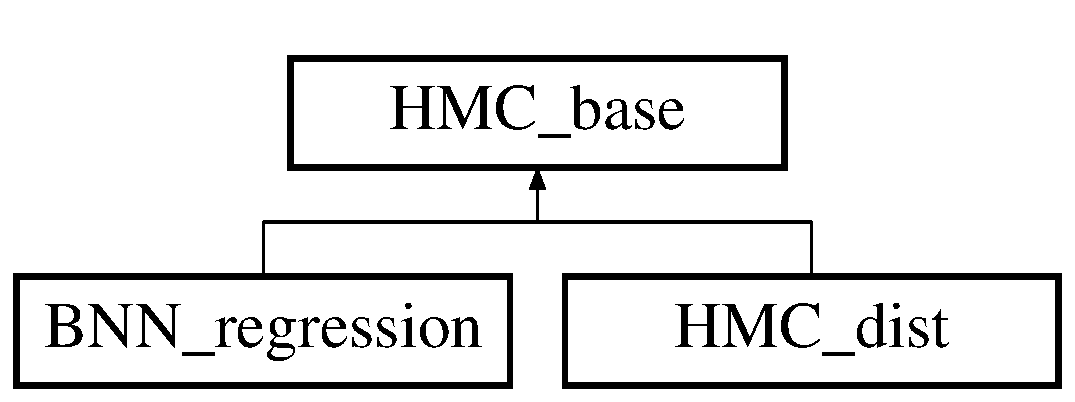
\includegraphics[height=2.000000cm]{class_h_m_c__base}
\end{center}
\end{figure}
\subsection*{Public Member Functions}
\begin{DoxyCompactItemize}
\item 
\hyperlink{class_h_m_c__base_a57549355656d15b406ffc0e89cb51be5}{H\-M\-C\-\_\-base} (int l, int n\-Params)
\item 
virtual \hyperlink{class_h_m_c__base_a27825ebbf86563706ed8f63b18367152}{$\sim$\-H\-M\-C\-\_\-base} ()
\item 
int \hyperlink{class_h_m_c__base_aa83e21d17eadcb907415a832560eb10d}{get\-N\-P} ()
\begin{DoxyCompactList}\small\item\em getter for N\-P variable in derived classes \end{DoxyCompactList}\item 
std\-::vector$<$ \hyperlink{define__type_8h_a9adf655d34223b34db3baff5c7ce420c}{H\-M\-C\-\_\-type} $>$ \& \hyperlink{class_h_m_c__base_a92b0fbc606f8c7c9e4e30f58f731921b}{it} (std\-::vector$<$ \hyperlink{define__type_8h_a9adf655d34223b34db3baff5c7ce420c}{H\-M\-C\-\_\-type} $>$ \&)
\begin{DoxyCompactList}\small\item\em one H\-M\-C iteration \end{DoxyCompactList}\item 
virtual \hyperlink{define__type_8h_a9adf655d34223b34db3baff5c7ce420c}{H\-M\-C\-\_\-type} \hyperlink{class_h_m_c__base_aab381fd0838b1a831906025b98a0c897}{U} (std\-::vector$<$ \hyperlink{define__type_8h_a9adf655d34223b34db3baff5c7ce420c}{H\-M\-C\-\_\-type} $>$ \&)=0
\begin{DoxyCompactList}\small\item\em calculate U \end{DoxyCompactList}\item 
virtual std\-::vector$<$ \hyperlink{define__type_8h_a9adf655d34223b34db3baff5c7ce420c}{H\-M\-C\-\_\-type} $>$ \hyperlink{class_h_m_c__base_acd263756d76e967e6ab678456cb88550}{del\-U} (std\-::vector$<$ \hyperlink{define__type_8h_a9adf655d34223b34db3baff5c7ce420c}{H\-M\-C\-\_\-type} $>$ \&)=0
\begin{DoxyCompactList}\small\item\em calculate d\-U $\ast$/ \end{DoxyCompactList}\end{DoxyCompactItemize}
\subsection*{Private Member Functions}
\begin{DoxyCompactItemize}
\item 
std\-::vector$<$ \hyperlink{define__type_8h_a9adf655d34223b34db3baff5c7ce420c}{H\-M\-C\-\_\-type} $>$ \hyperlink{class_h_m_c__base_a78e3fc2958f28c03b0af2dae57bb1902}{calc\-\_\-step} (std\-::vector$<$ \hyperlink{define__type_8h_a9adf655d34223b34db3baff5c7ce420c}{H\-M\-C\-\_\-type} $>$ \&\hyperlink{class_h_m_c__base_a9cb5e5ac7774b066976e6e9cac0dbfe8}{q})
\begin{DoxyCompactList}\small\item\em calculates step size each H\-M\-C iteration \end{DoxyCompactList}\end{DoxyCompactItemize}
\subsection*{Private Attributes}
\begin{DoxyCompactItemize}
\item 
int \hyperlink{class_h_m_c__base_a784a93d47df670ad254249233b6d81a1}{L}
\begin{DoxyCompactList}\small\item\em number of steps in one H\-M\-C iteration \end{DoxyCompactList}\item 
int \hyperlink{class_h_m_c__base_a204db698729d8f3ac18cbe8ce6257440}{N\-P}
\begin{DoxyCompactList}\small\item\em number of parameters \end{DoxyCompactList}\item 
\hyperlink{define__type_8h_a9adf655d34223b34db3baff5c7ce420c}{H\-M\-C\-\_\-type} \hyperlink{class_h_m_c__base_af1b25a6ca516eebc2385c6359daeff32}{Uq0}
\begin{DoxyCompactList}\small\item\em potential at current point \end{DoxyCompactList}\item 
std\-::vector$<$ \hyperlink{define__type_8h_a9adf655d34223b34db3baff5c7ce420c}{H\-M\-C\-\_\-type} $>$ \hyperlink{class_h_m_c__base_a9cb5e5ac7774b066976e6e9cac0dbfe8}{q}
\begin{DoxyCompactList}\small\item\em class parameters definition to avoid many re-\/allocations in loops \end{DoxyCompactList}\item 
std\-::vector$<$ \hyperlink{define__type_8h_a9adf655d34223b34db3baff5c7ce420c}{H\-M\-C\-\_\-type} $>$ \hyperlink{class_h_m_c__base_a138936eeaf2656aa5f2d51395c8e68f5}{p}
\begin{DoxyCompactList}\small\item\em class momentum definition to avoid many re-\/allocations in loops \end{DoxyCompactList}\end{DoxyCompactItemize}


\subsection{Detailed Description}
Base Hybrid Monte Carlo class. 





\begin{DoxyAuthor}{Author}
Michelle E. Perry 
\end{DoxyAuthor}
\begin{DoxyDate}{Date}
created 6/6/2013 updated 9/9/2013 
\end{DoxyDate}


Definition at line 14 of file H\-M\-C\-\_\-base.\-h.



\subsection{Constructor \& Destructor Documentation}
\hypertarget{class_h_m_c__base_a57549355656d15b406ffc0e89cb51be5}{\index{H\-M\-C\-\_\-base@{H\-M\-C\-\_\-base}!H\-M\-C\-\_\-base@{H\-M\-C\-\_\-base}}
\index{H\-M\-C\-\_\-base@{H\-M\-C\-\_\-base}!HMC_base@{H\-M\-C\-\_\-base}}
\subsubsection[{H\-M\-C\-\_\-base}]{\setlength{\rightskip}{0pt plus 5cm}H\-M\-C\-\_\-base\-::\-H\-M\-C\-\_\-base (
\begin{DoxyParamCaption}
\item[{int}]{l, }
\item[{int}]{n\-Params}
\end{DoxyParamCaption}
)\hspace{0.3cm}{\ttfamily [inline]}}}\label{class_h_m_c__base_a57549355656d15b406ffc0e89cb51be5}


Definition at line 22 of file H\-M\-C\-\_\-base.\-h.

\hypertarget{class_h_m_c__base_a27825ebbf86563706ed8f63b18367152}{\index{H\-M\-C\-\_\-base@{H\-M\-C\-\_\-base}!$\sim$\-H\-M\-C\-\_\-base@{$\sim$\-H\-M\-C\-\_\-base}}
\index{$\sim$\-H\-M\-C\-\_\-base@{$\sim$\-H\-M\-C\-\_\-base}!HMC_base@{H\-M\-C\-\_\-base}}
\subsubsection[{$\sim$\-H\-M\-C\-\_\-base}]{\setlength{\rightskip}{0pt plus 5cm}virtual H\-M\-C\-\_\-base\-::$\sim$\-H\-M\-C\-\_\-base (
\begin{DoxyParamCaption}
{}
\end{DoxyParamCaption}
)\hspace{0.3cm}{\ttfamily [inline]}, {\ttfamily [virtual]}}}\label{class_h_m_c__base_a27825ebbf86563706ed8f63b18367152}


Definition at line 29 of file H\-M\-C\-\_\-base.\-h.



\subsection{Member Function Documentation}
\hypertarget{class_h_m_c__base_a78e3fc2958f28c03b0af2dae57bb1902}{\index{H\-M\-C\-\_\-base@{H\-M\-C\-\_\-base}!calc\-\_\-step@{calc\-\_\-step}}
\index{calc\-\_\-step@{calc\-\_\-step}!HMC_base@{H\-M\-C\-\_\-base}}
\subsubsection[{calc\-\_\-step}]{\setlength{\rightskip}{0pt plus 5cm}std\-::vector$<$ {\bf H\-M\-C\-\_\-type} $>$ H\-M\-C\-\_\-base\-::calc\-\_\-step (
\begin{DoxyParamCaption}
\item[{std\-::vector$<$ {\bf H\-M\-C\-\_\-type} $>$ \&}]{q}
\end{DoxyParamCaption}
)\hspace{0.3cm}{\ttfamily [private]}}}\label{class_h_m_c__base_a78e3fc2958f28c03b0af2dae57bb1902}


calculates step size each H\-M\-C iteration 



Definition at line 7 of file H\-M\-C\-\_\-base.\-cc.



References N\-P, q, U(), and Uq0.



Referenced by it().

\hypertarget{class_h_m_c__base_acd263756d76e967e6ab678456cb88550}{\index{H\-M\-C\-\_\-base@{H\-M\-C\-\_\-base}!del\-U@{del\-U}}
\index{del\-U@{del\-U}!HMC_base@{H\-M\-C\-\_\-base}}
\subsubsection[{del\-U}]{\setlength{\rightskip}{0pt plus 5cm}virtual std\-::vector$<${\bf H\-M\-C\-\_\-type}$>$ H\-M\-C\-\_\-base\-::del\-U (
\begin{DoxyParamCaption}
\item[{std\-::vector$<$ {\bf H\-M\-C\-\_\-type} $>$ \&}]{}
\end{DoxyParamCaption}
)\hspace{0.3cm}{\ttfamily [pure virtual]}}}\label{class_h_m_c__base_acd263756d76e967e6ab678456cb88550}


calculate d\-U $\ast$/ 



Implemented in \hyperlink{class_b_n_n__regression_a779b2feff8192046b2670e80b88547ba}{B\-N\-N\-\_\-regression}, and \hyperlink{class_h_m_c__dist_a0fdfe885bac1033a4cccc8442b225937}{H\-M\-C\-\_\-dist}.



Referenced by it().

\hypertarget{class_h_m_c__base_aa83e21d17eadcb907415a832560eb10d}{\index{H\-M\-C\-\_\-base@{H\-M\-C\-\_\-base}!get\-N\-P@{get\-N\-P}}
\index{get\-N\-P@{get\-N\-P}!HMC_base@{H\-M\-C\-\_\-base}}
\subsubsection[{get\-N\-P}]{\setlength{\rightskip}{0pt plus 5cm}int H\-M\-C\-\_\-base\-::get\-N\-P (
\begin{DoxyParamCaption}
{}
\end{DoxyParamCaption}
)}}\label{class_h_m_c__base_aa83e21d17eadcb907415a832560eb10d}


getter for N\-P variable in derived classes 



Definition at line 151 of file H\-M\-C\-\_\-base.\-cc.



References N\-P.



Referenced by B\-N\-N\-\_\-regression\-::\-U().

\hypertarget{class_h_m_c__base_a92b0fbc606f8c7c9e4e30f58f731921b}{\index{H\-M\-C\-\_\-base@{H\-M\-C\-\_\-base}!it@{it}}
\index{it@{it}!HMC_base@{H\-M\-C\-\_\-base}}
\subsubsection[{it}]{\setlength{\rightskip}{0pt plus 5cm}std\-::vector$<$ {\bf H\-M\-C\-\_\-type} $>$ \& H\-M\-C\-\_\-base\-::it (
\begin{DoxyParamCaption}
\item[{std\-::vector$<$ {\bf H\-M\-C\-\_\-type} $>$ \&}]{q0}
\end{DoxyParamCaption}
)}}\label{class_h_m_c__base_a92b0fbc606f8c7c9e4e30f58f731921b}


one H\-M\-C iteration 

$<$ Uq0 calculated in this function 

Definition at line 46 of file H\-M\-C\-\_\-base.\-cc.



References calc\-\_\-step(), del\-U(), L, N\-P, p, q, U(), and Uq0.

\hypertarget{class_h_m_c__base_aab381fd0838b1a831906025b98a0c897}{\index{H\-M\-C\-\_\-base@{H\-M\-C\-\_\-base}!U@{U}}
\index{U@{U}!HMC_base@{H\-M\-C\-\_\-base}}
\subsubsection[{U}]{\setlength{\rightskip}{0pt plus 5cm}virtual {\bf H\-M\-C\-\_\-type} H\-M\-C\-\_\-base\-::\-U (
\begin{DoxyParamCaption}
\item[{std\-::vector$<$ {\bf H\-M\-C\-\_\-type} $>$ \&}]{}
\end{DoxyParamCaption}
)\hspace{0.3cm}{\ttfamily [pure virtual]}}}\label{class_h_m_c__base_aab381fd0838b1a831906025b98a0c897}


calculate U 



Implemented in \hyperlink{class_b_n_n__regression_a57303ef1ca25e08c7489fb5095f23527}{B\-N\-N\-\_\-regression}, and \hyperlink{class_h_m_c__dist_ab536db252ec2926399e030b576a47f22}{H\-M\-C\-\_\-dist}.



Referenced by calc\-\_\-step(), and it().



\subsection{Field Documentation}
\hypertarget{class_h_m_c__base_a784a93d47df670ad254249233b6d81a1}{\index{H\-M\-C\-\_\-base@{H\-M\-C\-\_\-base}!L@{L}}
\index{L@{L}!HMC_base@{H\-M\-C\-\_\-base}}
\subsubsection[{L}]{\setlength{\rightskip}{0pt plus 5cm}int H\-M\-C\-\_\-base\-::\-L\hspace{0.3cm}{\ttfamily [private]}}}\label{class_h_m_c__base_a784a93d47df670ad254249233b6d81a1}


number of steps in one H\-M\-C iteration 



Definition at line 15 of file H\-M\-C\-\_\-base.\-h.



Referenced by it().

\hypertarget{class_h_m_c__base_a204db698729d8f3ac18cbe8ce6257440}{\index{H\-M\-C\-\_\-base@{H\-M\-C\-\_\-base}!N\-P@{N\-P}}
\index{N\-P@{N\-P}!HMC_base@{H\-M\-C\-\_\-base}}
\subsubsection[{N\-P}]{\setlength{\rightskip}{0pt plus 5cm}int H\-M\-C\-\_\-base\-::\-N\-P\hspace{0.3cm}{\ttfamily [private]}}}\label{class_h_m_c__base_a204db698729d8f3ac18cbe8ce6257440}


number of parameters 



Definition at line 16 of file H\-M\-C\-\_\-base.\-h.



Referenced by calc\-\_\-step(), get\-N\-P(), and it().

\hypertarget{class_h_m_c__base_a138936eeaf2656aa5f2d51395c8e68f5}{\index{H\-M\-C\-\_\-base@{H\-M\-C\-\_\-base}!p@{p}}
\index{p@{p}!HMC_base@{H\-M\-C\-\_\-base}}
\subsubsection[{p}]{\setlength{\rightskip}{0pt plus 5cm}std\-::vector$<${\bf H\-M\-C\-\_\-type}$>$ H\-M\-C\-\_\-base\-::p\hspace{0.3cm}{\ttfamily [private]}}}\label{class_h_m_c__base_a138936eeaf2656aa5f2d51395c8e68f5}


class momentum definition to avoid many re-\/allocations in loops 



Definition at line 20 of file H\-M\-C\-\_\-base.\-h.



Referenced by it().

\hypertarget{class_h_m_c__base_a9cb5e5ac7774b066976e6e9cac0dbfe8}{\index{H\-M\-C\-\_\-base@{H\-M\-C\-\_\-base}!q@{q}}
\index{q@{q}!HMC_base@{H\-M\-C\-\_\-base}}
\subsubsection[{q}]{\setlength{\rightskip}{0pt plus 5cm}std\-::vector$<${\bf H\-M\-C\-\_\-type}$>$ H\-M\-C\-\_\-base\-::q\hspace{0.3cm}{\ttfamily [private]}}}\label{class_h_m_c__base_a9cb5e5ac7774b066976e6e9cac0dbfe8}


class parameters definition to avoid many re-\/allocations in loops 



Definition at line 19 of file H\-M\-C\-\_\-base.\-h.



Referenced by calc\-\_\-step(), H\-M\-C\-\_\-dist\-::\-F\-D(), and it().

\hypertarget{class_h_m_c__base_af1b25a6ca516eebc2385c6359daeff32}{\index{H\-M\-C\-\_\-base@{H\-M\-C\-\_\-base}!Uq0@{Uq0}}
\index{Uq0@{Uq0}!HMC_base@{H\-M\-C\-\_\-base}}
\subsubsection[{Uq0}]{\setlength{\rightskip}{0pt plus 5cm}{\bf H\-M\-C\-\_\-type} H\-M\-C\-\_\-base\-::\-Uq0\hspace{0.3cm}{\ttfamily [private]}}}\label{class_h_m_c__base_af1b25a6ca516eebc2385c6359daeff32}


potential at current point 



Definition at line 17 of file H\-M\-C\-\_\-base.\-h.



Referenced by calc\-\_\-step(), and it().



The documentation for this class was generated from the following files\-:\begin{DoxyCompactItemize}
\item 
include/\hyperlink{_h_m_c__base_8h}{H\-M\-C\-\_\-base.\-h}\item 
src/\hyperlink{_h_m_c__base_8cc}{H\-M\-C\-\_\-base.\-cc}\end{DoxyCompactItemize}

\hypertarget{class_h_m_c__dist}{\section{H\-M\-C\-\_\-dist Class Reference}
\label{class_h_m_c__dist}\index{H\-M\-C\-\_\-dist@{H\-M\-C\-\_\-dist}}
}


probability distribution class  




{\ttfamily \#include \char`\"{}H\-M\-C\-\_\-dist.\-h\char`\"{}}

Inheritance diagram for H\-M\-C\-\_\-dist\-:\begin{figure}[H]
\begin{center}
\leavevmode
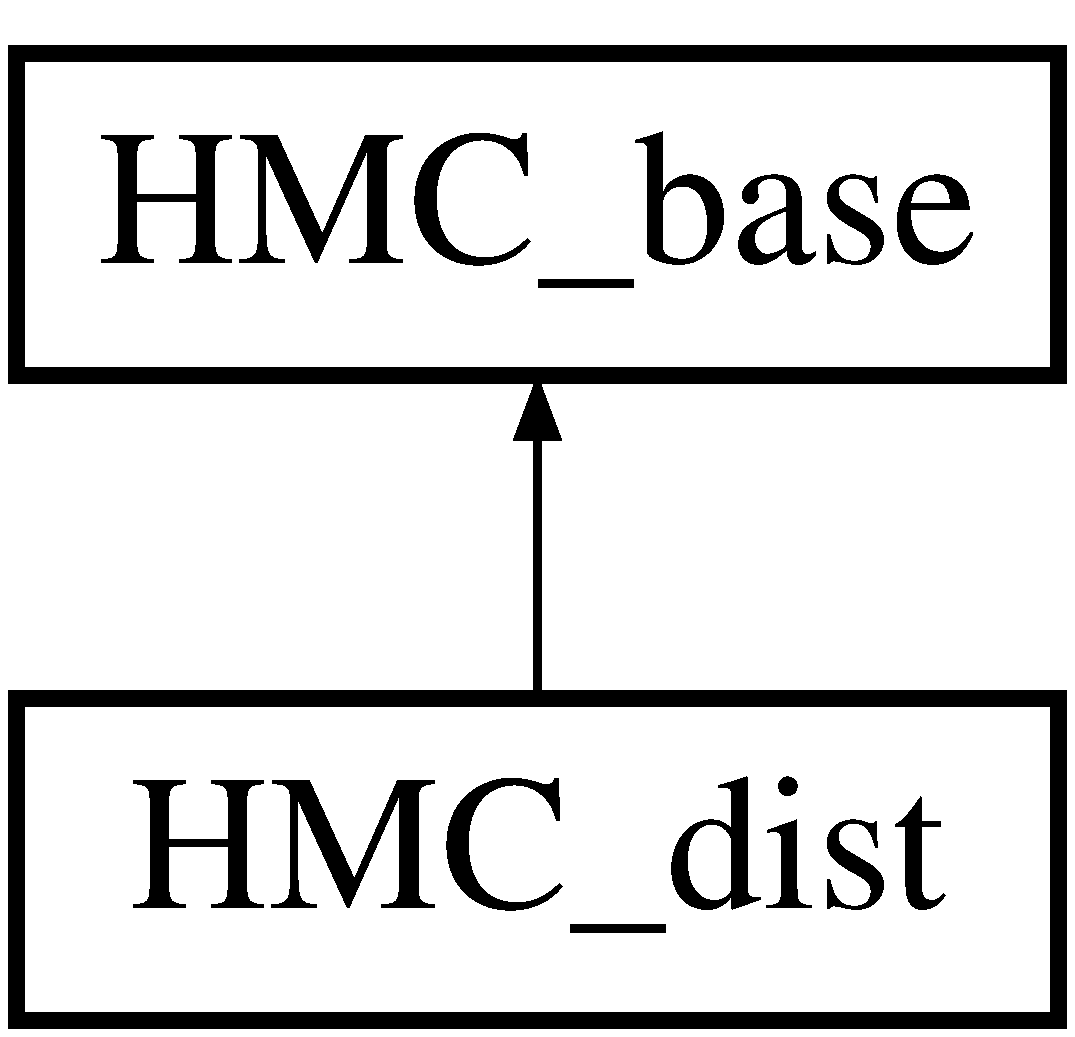
\includegraphics[height=2.000000cm]{class_h_m_c__dist}
\end{center}
\end{figure}
\subsection*{Public Member Functions}
\begin{DoxyCompactItemize}
\item 
\hyperlink{class_h_m_c__dist_a62e12ed5444505af3ffae0e6971845e2}{H\-M\-C\-\_\-dist} (int l, int n\-Params)
\item 
virtual \hyperlink{define__type_8h_a9adf655d34223b34db3baff5c7ce420c}{H\-M\-C\-\_\-type} \hyperlink{class_h_m_c__dist_ab536db252ec2926399e030b576a47f22}{U} (std\-::vector$<$ \hyperlink{define__type_8h_a9adf655d34223b34db3baff5c7ce420c}{H\-M\-C\-\_\-type} $>$ \&)
\begin{DoxyCompactList}\small\item\em U = -\/ln(P(q)) \end{DoxyCompactList}\item 
virtual std\-::vector$<$ \hyperlink{define__type_8h_a9adf655d34223b34db3baff5c7ce420c}{H\-M\-C\-\_\-type} $>$ \hyperlink{class_h_m_c__dist_a0fdfe885bac1033a4cccc8442b225937}{del\-U} (std\-::vector$<$ \hyperlink{define__type_8h_a9adf655d34223b34db3baff5c7ce420c}{H\-M\-C\-\_\-type} $>$ \&)
\begin{DoxyCompactList}\small\item\em calculate d\-U $\ast$/ \end{DoxyCompactList}\item 
std\-::vector$<$ \hyperlink{define__type_8h_a9adf655d34223b34db3baff5c7ce420c}{H\-M\-C\-\_\-type} $>$ \hyperlink{class_h_m_c__dist_adf7687e9feb76025e5cd3095c357cc10}{F\-D} (std\-::vector$<$ \hyperlink{define__type_8h_a9adf655d34223b34db3baff5c7ce420c}{H\-M\-C\-\_\-type} $>$ \&\hyperlink{class_h_m_c__base_a9cb5e5ac7774b066976e6e9cac0dbfe8}{q})
\end{DoxyCompactItemize}


\subsection{Detailed Description}
probability distribution class 





\begin{DoxyAuthor}{Author}
Michelle E. Perry 
\end{DoxyAuthor}
\begin{DoxyDate}{Date}
created 21/2/13 updated 
\end{DoxyDate}


Definition at line 15 of file H\-M\-C\-\_\-dist.\-h.



\subsection{Constructor \& Destructor Documentation}
\hypertarget{class_h_m_c__dist_a62e12ed5444505af3ffae0e6971845e2}{\index{H\-M\-C\-\_\-dist@{H\-M\-C\-\_\-dist}!H\-M\-C\-\_\-dist@{H\-M\-C\-\_\-dist}}
\index{H\-M\-C\-\_\-dist@{H\-M\-C\-\_\-dist}!HMC_dist@{H\-M\-C\-\_\-dist}}
\subsubsection[{H\-M\-C\-\_\-dist}]{\setlength{\rightskip}{0pt plus 5cm}H\-M\-C\-\_\-dist\-::\-H\-M\-C\-\_\-dist (
\begin{DoxyParamCaption}
\item[{int}]{l, }
\item[{int}]{n\-Params}
\end{DoxyParamCaption}
)\hspace{0.3cm}{\ttfamily [inline]}}}\label{class_h_m_c__dist_a62e12ed5444505af3ffae0e6971845e2}


Definition at line 17 of file H\-M\-C\-\_\-dist.\-h.



\subsection{Member Function Documentation}
\hypertarget{class_h_m_c__dist_a0fdfe885bac1033a4cccc8442b225937}{\index{H\-M\-C\-\_\-dist@{H\-M\-C\-\_\-dist}!del\-U@{del\-U}}
\index{del\-U@{del\-U}!HMC_dist@{H\-M\-C\-\_\-dist}}
\subsubsection[{del\-U}]{\setlength{\rightskip}{0pt plus 5cm}std\-::vector$<$ {\bf H\-M\-C\-\_\-type} $>$ H\-M\-C\-\_\-dist\-::del\-U (
\begin{DoxyParamCaption}
\item[{std\-::vector$<$ {\bf H\-M\-C\-\_\-type} $>$ \&}]{}
\end{DoxyParamCaption}
)\hspace{0.3cm}{\ttfamily [virtual]}}}\label{class_h_m_c__dist_a0fdfe885bac1033a4cccc8442b225937}


calculate d\-U $\ast$/ 



Implements \hyperlink{class_h_m_c__base_acd263756d76e967e6ab678456cb88550}{H\-M\-C\-\_\-base}.



Definition at line 39 of file multidimprob.\-cc.



References F\-D().

\hypertarget{class_h_m_c__dist_adf7687e9feb76025e5cd3095c357cc10}{\index{H\-M\-C\-\_\-dist@{H\-M\-C\-\_\-dist}!F\-D@{F\-D}}
\index{F\-D@{F\-D}!HMC_dist@{H\-M\-C\-\_\-dist}}
\subsubsection[{F\-D}]{\setlength{\rightskip}{0pt plus 5cm}std\-::vector$<${\bf H\-M\-C\-\_\-type}$>$ H\-M\-C\-\_\-dist\-::\-F\-D (
\begin{DoxyParamCaption}
\item[{std\-::vector$<$ {\bf H\-M\-C\-\_\-type} $>$ \&}]{q}
\end{DoxyParamCaption}
)\hspace{0.3cm}{\ttfamily [inline]}}}\label{class_h_m_c__dist_adf7687e9feb76025e5cd3095c357cc10}


Definition at line 25 of file H\-M\-C\-\_\-dist.\-h.



References H\-M\-C\-\_\-base\-::q, and U().



Referenced by del\-U().

\hypertarget{class_h_m_c__dist_ab536db252ec2926399e030b576a47f22}{\index{H\-M\-C\-\_\-dist@{H\-M\-C\-\_\-dist}!U@{U}}
\index{U@{U}!HMC_dist@{H\-M\-C\-\_\-dist}}
\subsubsection[{U}]{\setlength{\rightskip}{0pt plus 5cm}{\bf H\-M\-C\-\_\-type} H\-M\-C\-\_\-dist\-::\-U (
\begin{DoxyParamCaption}
\item[{std\-::vector$<$ {\bf H\-M\-C\-\_\-type} $>$ \&}]{q}
\end{DoxyParamCaption}
)\hspace{0.3cm}{\ttfamily [virtual]}}}\label{class_h_m_c__dist_ab536db252ec2926399e030b576a47f22}


U = -\/ln(P(q)) 



Implements \hyperlink{class_h_m_c__base_aab381fd0838b1a831906025b98a0c897}{H\-M\-C\-\_\-base}.



Definition at line 5 of file multidimprob.\-cc.



Referenced by F\-D().



The documentation for this class was generated from the following files\-:\begin{DoxyCompactItemize}
\item 
include/\hyperlink{_h_m_c__dist_8h}{H\-M\-C\-\_\-dist.\-h}\item 
src/\hyperlink{multidimprob_8cc}{multidimprob.\-cc}\end{DoxyCompactItemize}

\chapter{File Documentation}
\hypertarget{_b_n_n__regression_8h}{\section{include/\-B\-N\-N\-\_\-regression.h File Reference}
\label{_b_n_n__regression_8h}\index{include/\-B\-N\-N\-\_\-regression.\-h@{include/\-B\-N\-N\-\_\-regression.\-h}}
}
{\ttfamily \#include \char`\"{}H\-M\-C\-\_\-base.\-h\char`\"{}}\\*
{\ttfamily \#include $<$iostream$>$}\\*
\subsection*{Data Structures}
\begin{DoxyCompactItemize}
\item 
class \hyperlink{class_b_n_n__regression}{B\-N\-N\-\_\-regression}
\begin{DoxyCompactList}\small\item\em B\-N\-N functional approximation class. \end{DoxyCompactList}\end{DoxyCompactItemize}

\hypertarget{define__type_8h}{\section{include/define\-\_\-type.h File Reference}
\label{define__type_8h}\index{include/define\-\_\-type.\-h@{include/define\-\_\-type.\-h}}
}
\subsection*{Typedefs}
\begin{DoxyCompactItemize}
\item 
typedef float \hyperlink{define__type_8h_a9adf655d34223b34db3baff5c7ce420c}{H\-M\-C\-\_\-type}
\end{DoxyCompactItemize}


\subsection{Typedef Documentation}
\hypertarget{define__type_8h_a9adf655d34223b34db3baff5c7ce420c}{\index{define\-\_\-type.\-h@{define\-\_\-type.\-h}!H\-M\-C\-\_\-type@{H\-M\-C\-\_\-type}}
\index{H\-M\-C\-\_\-type@{H\-M\-C\-\_\-type}!define_type.h@{define\-\_\-type.\-h}}
\subsubsection[{H\-M\-C\-\_\-type}]{\setlength{\rightskip}{0pt plus 5cm}typedef float {\bf H\-M\-C\-\_\-type}}}\label{define__type_8h_a9adf655d34223b34db3baff5c7ce420c}


Definition at line 4 of file define\-\_\-type.\-h.


\hypertarget{_h_m_c__base_8h}{\section{include/\-H\-M\-C\-\_\-base.h File Reference}
\label{_h_m_c__base_8h}\index{include/\-H\-M\-C\-\_\-base.\-h@{include/\-H\-M\-C\-\_\-base.\-h}}
}
{\ttfamily \#include $<$vector$>$}\\*
{\ttfamily \#include \char`\"{}define\-\_\-type.\-h\char`\"{}}\\*
\subsection*{Data Structures}
\begin{DoxyCompactItemize}
\item 
class \hyperlink{class_h_m_c__base}{H\-M\-C\-\_\-base}
\begin{DoxyCompactList}\small\item\em Base Hybrid Monte Carlo class. \end{DoxyCompactList}\end{DoxyCompactItemize}

\hypertarget{_h_m_c__dist_8h}{\section{include/\-H\-M\-C\-\_\-dist.h File Reference}
\label{_h_m_c__dist_8h}\index{include/\-H\-M\-C\-\_\-dist.\-h@{include/\-H\-M\-C\-\_\-dist.\-h}}
}
{\ttfamily \#include \char`\"{}define\-\_\-type.\-h\char`\"{}}\\*
{\ttfamily \#include \char`\"{}H\-M\-C\-\_\-base.\-h\char`\"{}}\\*
\subsection*{Data Structures}
\begin{DoxyCompactItemize}
\item 
class \hyperlink{class_h_m_c__dist}{H\-M\-C\-\_\-dist}
\begin{DoxyCompactList}\small\item\em probability distribution class \end{DoxyCompactList}\end{DoxyCompactItemize}

\hypertarget{_b_n_n__regression_8cc}{\section{src/\-B\-N\-N\-\_\-regression.cc File Reference}
\label{_b_n_n__regression_8cc}\index{src/\-B\-N\-N\-\_\-regression.\-cc@{src/\-B\-N\-N\-\_\-regression.\-cc}}
}
{\ttfamily \#include \char`\"{}B\-N\-N\-\_\-regression.\-h\char`\"{}}\\*
{\ttfamily \#include $<$math.\-h$>$}\\*
{\ttfamily \#include $<$iostream$>$}\\*
{\ttfamily \#include $<$iomanip$>$}\\*


\subsection{Detailed Description}




\begin{DoxyAuthor}{Author}
Michelle E. Perry 
\end{DoxyAuthor}
\begin{DoxyDate}{Date}
created 25/2/2013 updated 9/9/2013 
\end{DoxyDate}


Definition in file \hyperlink{_b_n_n__regression_8cc_source}{B\-N\-N\-\_\-regression.\-cc}.


\hypertarget{_h_m_c_8cxx}{\section{src/\-H\-M\-C.cxx File Reference}
\label{_h_m_c_8cxx}\index{src/\-H\-M\-C.\-cxx@{src/\-H\-M\-C.\-cxx}}
}
{\ttfamily \#include $<$cmath$>$}\\*
{\ttfamily \#include $<$iostream$>$}\\*
{\ttfamily \#include \char`\"{}H\-M\-C.\-h\char`\"{}}\\*
{\ttfamily \#include \char`\"{}prob\-Dist.\-h\char`\"{}}\\*
\subsection*{Functions}
\begin{DoxyCompactItemize}
\item 
std\-::vector$<$ float $>$ \hyperlink{_h_m_c_8cxx_ae79adca1291a0ea216719698061d2282}{H\-M\-C} (float eps, int L, std\-::vector$<$ float $>$ \&q0)
\end{DoxyCompactItemize}


\subsection{Function Documentation}
\hypertarget{_h_m_c_8cxx_ae79adca1291a0ea216719698061d2282}{\index{H\-M\-C.\-cxx@{H\-M\-C.\-cxx}!H\-M\-C@{H\-M\-C}}
\index{H\-M\-C@{H\-M\-C}!HMC.cxx@{H\-M\-C.\-cxx}}
\subsubsection[{H\-M\-C}]{\setlength{\rightskip}{0pt plus 5cm}std\-::vector$<$float$>$ H\-M\-C (
\begin{DoxyParamCaption}
\item[{float}]{eps, }
\item[{int}]{L, }
\item[{std\-::vector$<$ float $>$ \&}]{q0}
\end{DoxyParamCaption}
)}}\label{_h_m_c_8cxx_ae79adca1291a0ea216719698061d2282}


Definition at line 6 of file H\-M\-C.\-cxx.


\hypertarget{_h_m_c__base_8cc}{\section{src/\-H\-M\-C\-\_\-base.cc File Reference}
\label{_h_m_c__base_8cc}\index{src/\-H\-M\-C\-\_\-base.\-cc@{src/\-H\-M\-C\-\_\-base.\-cc}}
}
{\ttfamily \#include $<$cmath$>$}\\*
{\ttfamily \#include $<$cassert$>$}\\*
{\ttfamily \#include \char`\"{}H\-M\-C\-\_\-base.\-h\char`\"{}}\\*
{\ttfamily \#include \char`\"{}define\-\_\-type.\-h\char`\"{}}\\*
{\ttfamily \#include $<$iostream$>$}\\*

\hypertarget{multidimprob_8cc}{\section{src/multidimprob.cc File Reference}
\label{multidimprob_8cc}\index{src/multidimprob.\-cc@{src/multidimprob.\-cc}}
}
{\ttfamily \#include \char`\"{}H\-M\-C\-\_\-dist.\-h\char`\"{}}\\*
{\ttfamily \#include $<$math.\-h$>$}\\*

%--- End generated contents ---

% Index
\newpage
\phantomsection
\addcontentsline{toc}{part}{Index}
\printindex

\end{document}
